\section{Teilaufgabe 22}
\begin{aufgabe}
    Programmieren Sie den ganzen Regelkreis mit Simulink.
\end{aufgabe}
\begin{figure}[h!]
    \centering
    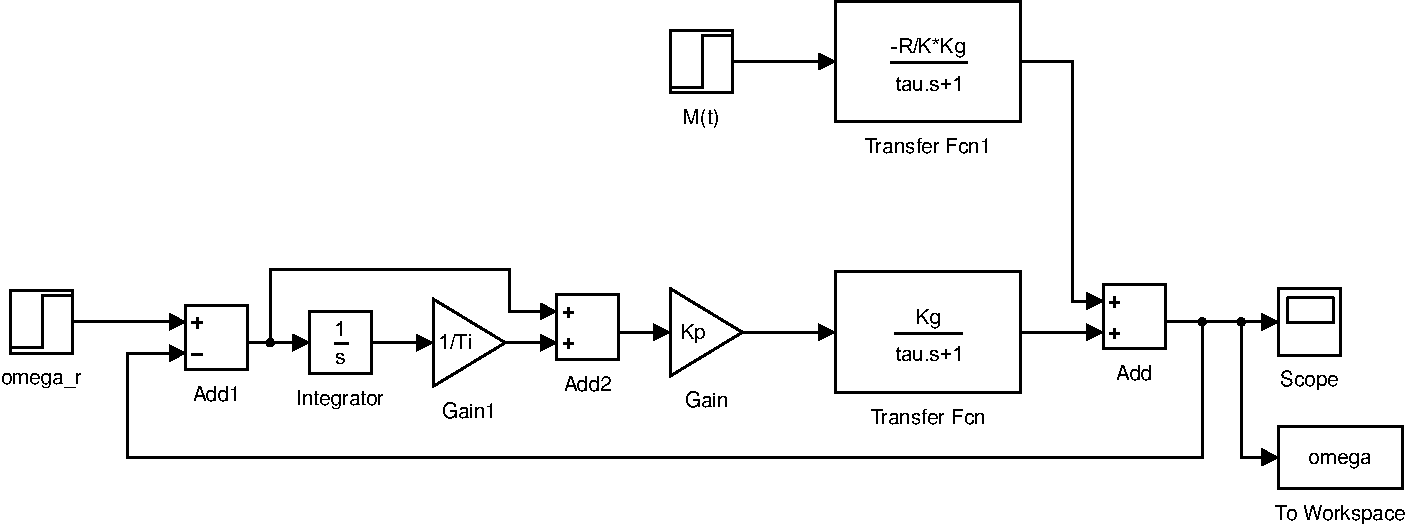
\includegraphics[width=0.6\textwidth]{22/regler_pi.pdf}
    \caption{Regler in Simulink}
    \label{fig:22}
\end{figure}
\begin{figure}[h!]
    \centering
    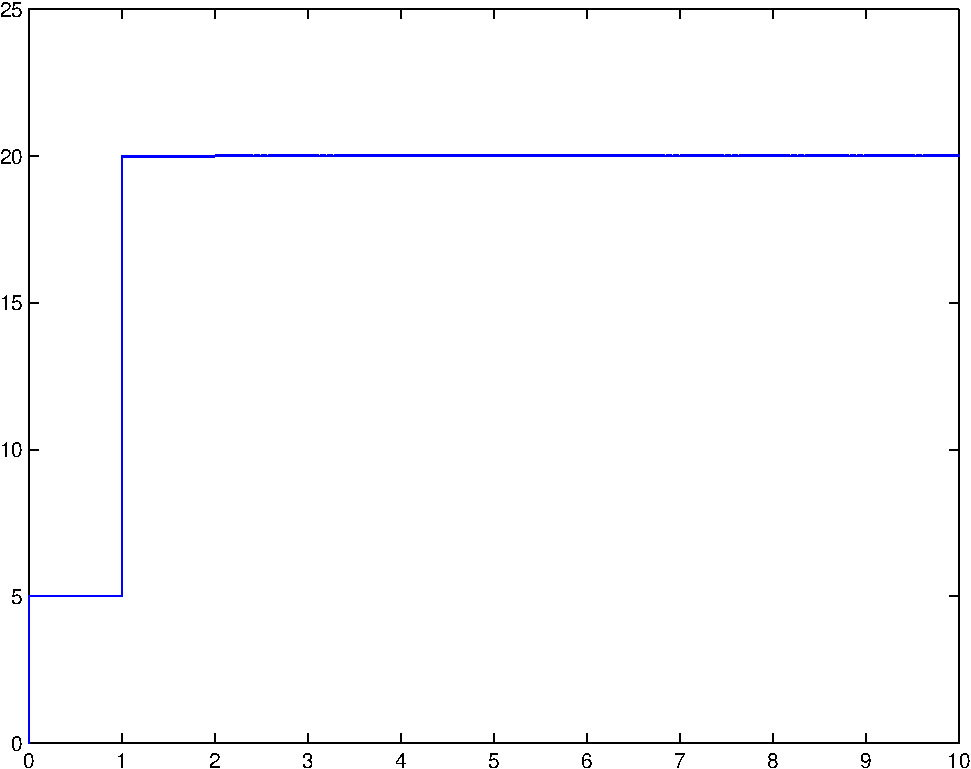
\includegraphics[width=0.6\textwidth]{22/regler_pi_plot.pdf}
    \caption{Simulationsergebnis}
    \label{fig:22plot}
\end{figure}
\lstinputlisting{22/regler_pi.m}
